The design, implementation and application of a concept for
object-orientated in finite element analysis of multi-field
problems is presented in this paper.
%
The basic idea of this concept is that the underlying governing
equations of porous media mechanics can be classified into
different types of partial differential equations (PDEs). In
principle, equal types of PDEs for diverse physical problems
differ only in material coefficients.
%
Local element matrices and vectors arising from the finite element
discretization of the PDEs are categorized into several types,
regardless of which physical problem they belong to (i.e. fluid flow, mass and
heat transport or deformation processes).
%
Element (ELE) objects are introduced to carry out the local
assembly of the algebraic equations. The object-orientation
includes a strict encapsulation of geometrical (GEO), topological
(MSH), process-related (FEM) data and methods of element objects.
%
Geometric entities of an element such as nodes, edges, faces and
 neighbors are abstracted into corresponding geometric element
objects (ELE-GEO). The relationships among these geometric
entities form the topology of element meshes (ELE-MSH).
%
Finite element objects (ELE-FEM) are presented for the local
element calculations, in which each classification type of the 
matrices and vectors is computed by a unique function. These
element functions are able to deal with different element types
(lines, triangles, quadrilaterals, tetrahedra, prisms, hexhedra) by 
automatically choosing the related element interpolation
functions.
%
For each process of a multi-field problem, only a single instance of 
the finite element object is required. The element objects provide a 
flexible coding environment for multi-field problems with different 
element types. Here, the C++ implementations of the objects are given and 
described in detail.
%
The efficiency of the new element objects is demonstrated by
several test cases dealing with thermo-hydro-mechanical (THM)
coupled problems for geotechnical applications.

\section{Introduction}

%\subsection{Motivation}
The numerical analysis of complex multi-field problems is an 
important issue for many engineering problems. A representative 
example is nuclear waste disposal. Nuclear waste repositories are 
constructed in deep geologic underground. Normally, the radioactive 
waste will generate heat for a long period of time with temperatures 
over 100$^\circ$C. Possibly, ground water \rev{flow} may be 
developed and gas will be produced due to the heating of the ground 
water. The coupling of thermal and hydraulic processes can cause 
mechanical damage in the near field of the host rock mass. To assess 
the safety of the underground repositories, the problem needs to be 
addressed as a thermo-hydro-mechanical
 (THM) coupled problem \cite{{LeSch:98},{deBoer:00},{deBoer:05},{StHuJi:02},{EhBl:02},{KolEtAl:2004a},{OKJO:04}}.
Although some commercial tools are already available, there is a 
tremendous demand in the development of fully coupled THM codes. 
Existing concepts couple obtainable codes which are specialized to 
hydraulic, mechanic or deformation problems. The coupling is then 
realized by data exchange between these codes. This procedure causes 
a rigorous restriction of the modeling of coupling phenomena. In 
this work we present a finite element class which can deal with 
thermal, hydraulic as well as mechanic problems.

%\subsection{Programming paradigms}
For the programming paradigms, there are two alternatives for finite 
element code design and development, i.e. procedure-oriented or 
object-oriented. The former does not encapsulate data and methods 
manipulating the data together, the latter does encapsulate data and 
methods and provides regulated communication between data and 
methods to perform tasks \cite{{StrB:00},{Budd:01}}. The object 
oriented paradigm \rev{facilitates} data abstract with its 
capabilities of data encapsulation, polymorphism and inheritance. 
Therefore, it provides us a easy way to develop and to maintain a 
code. This is a reason why more and more researchers are attracted 
to shift from using procedure oriented to  OOP paradigm in numerical 
analysis. Other reasons for its popularity is that software of 
increasing complexity has to be developed by permanently increasing 
programmer teams. OOP has significant advantages by allowing rapid 
software development through \rev{capsulation, inheritance and 
polymorph of data and methods}. 
%
The advantages of object-oriented programming for the development of 
engineering software was described in detail by \cite{Fen:90}.

%\subsection{History}
Although the fundamentals of object-orientated programming (OOP)
were established in the 1960s, it remains a very important concept
to face challenges in scientific computation, such as the solution
of coupled multi-field problems.
%
One of the first applications of the object-oriented paradigm to 
finite element analysis was published in 1990 \cite{FOFOST:90}, 
where essential components of finite element methods such as 
elements, nodes and materials were abstracted into classes. More 
efforts have been made by 
\cite{{FilDev:91},{Mack:92},{ZimYve:92},{YveZim:92}, 
{YveZim:93},{PidHud:93}, {RapKris:93}} in order to demonstrated the 
advantages of OOP over the procedure oriented programming. Moreover, 
the applications to many different physical problems have been 
investigated, such as linear stress analysis 
\cite{{ZimYve:92},{YveZim:92}, {YveZim:93}}, hypersonic shock waves 
\cite{BudPee:93}, structural dynamics \cite{PidHudli:93}, 2D Mises 
plasticity \cite{MenZim:93}, linear static problems 
\cite{{AdeFu:93},{AdeFu:95}}, electro-magnetics \cite{SilMes:94}, 
solidification process \cite{SaZa:99},  heat transfer as well as 
topological buildup \cite{RihKro94}. A process-oriented approach for 
the solution of multi-field problems in porous media is presented in 
\cite{{KolBau:04},{KolEtAl:2004a}}. Numerical objects for algebraic 
calculations in finite element analysis have been developed by 
\cite{{Scholz:92},{ZegHanAit:94},{LuWCD:95}}. \rev{In order to 
provide an automatic coding environment for finite element analysis, 
a symbolic code development concept is presented for the weak forms 
arising from the partial differential 
equations \cite{{ZimEyh:96},{EyhZim:96},{EyhZim:98},{EyhZim:01}}}.

Object design is the fundamental step in object-oriented
programming. The utilization of OOP to finite element analysis is
mainly focused on three aspects: (1) pre/post processing such as
mesh generation and graphical user interface, (2) linear algebra
and (3) finite element methods. In all these aspects, the core
object is the element object. The design of element objects is
associated with other objects corresponding to material
properties, numerical methods, local geometry and topology of
element etc. Specific material objects are described in the
most of references cited above.

In this part we present the design, implementation and application of 
object-orientation in finite element analysis for multi-physics 
problems. The development of a universal object for local 
finite element calculation and assembly is able to 
cope with different kinds of physical problems (i.e. different types 
of partial differential equations) and is, in particular, designed 
for strongly coupled problems. Additionally, object-orientation is used 
in description of mesh topology for the global assembly of system 
equations. The description of the programming semantics of these 
objects is given in C++. All the developments of this work are 
conducted within the framework of the scientific 
software project OGS \cite{geosys}. The the OO-FEM concept is verified by 
numerous test cases dealing with thermo-hydro-mechanical (THM) 
coupled problems in geotechnical as well as hydrological applications (Parts II and III of this book.)

\section{Object-orientation in finite element analysis}
\label{sec:ovl}

Almost all numerical methods eventually have to deal with the
solution of algebraic equation systems. The basic algorithms for
the discretization of partial differential equations (PDEs)
resulting from the initial-boundary-value-problems (IBVPs) of
continuum mechanics can be generalized in principle as follows:
time discretization, calculation of problem-specific node (finite
difference method - FDM), element (finite element method - FEM),
volume (finite volume method - FVM) contributions, incorporating
initial and boundary conditions, assembling and solving the resulting
equation system. For non-linear problems iteration schemes, such
as Picard or Newton methods, have to be used.

The general solution algorithm for the finite element method is
given in Table \ref{tab:alg1}.

\newpage

%.........................................................................
\rule{\textwidth}{0.25mm}
\begin{enumerate}
  \item Domain \rev{discretization} ( i.e. mesh generation): Creation of individual
geometric elements (e.g. triangles, tetrahedra) and their
topological relationships (mesh topology).
  \item Local element assembly: Depending on PDE type (section
\ref{sec:fem}) all element matrices and vectors have to be
computed. The element integration requires geometric operations
such as interpolation with shape functions, calculation of inverse
Jacobians and determinants. Additionally material functions have
to be computed in Gauss points. Material functions can depend on
field variables.
  \begin{itemize}
    \item Geometric element operations (shape functions, Jacobian),
    \item Material parameter calculation at Gauss points,
  \end{itemize}
  \item Global assembly of the algebraic equation $\mathbf{Ax=b}$: The local element
  entries are assembled into the global system matrix $\mathbf A$ and global
  RHS vector $\mathbf b$. The equations systems is established after \rev{incorporating} boundary conditions and source/sink terms.

  \begin{itemize}
    \item Assembly of system matrix $\mathbf A$ (including incorporation of boundary
    conditions),
    \item Assembly of RHS vector $\mathbf b$ (including incorporation of source/sink
    terms),
  \end{itemize}
  \item Solving the system equations,
  \item Iterative methods to handle non-linearities,
  \item Iterative methods to handle couplings (partitioned and monolithic schemes).
\end{enumerate}
\rule{\textwidth}{0.25mm}
\begin{table}[H]
\begin{tabular}{c}
\end{tabular}
 \caption{General solution procedure of the finite element method}
 \label{tab:alg1}
\end{table}

%.........................................................................
The implementation of the general solution algorithm for multi-field
IBVPs according to Table \ref{tab:alg1} is illustrated in Fig.
\ref{fig:alg}. The time loop represents time discretization. Within
the time loop, specified physical processes (e.g. flow, transport,
deformation) are solved using the finite element method (left box).
The solution procedure of each process is unique (middle box). The
basic part is the calculation and assembly of element contribution
(right box).

%.........................................................................
Based on above described general solution algorithm for
multi-field IBVPs, the fundamental concept of object-orientation
in finite element analysis is the generalization of
\begin{itemize}
    \item Process (PCS) types (section \ref{sec:pcs}),
    \item Equation (PDE) types (section \ref{sec:pde}),
    \item Element (ELE) types (section \ref{sec:ele}).
\end{itemize}

\begin{figure}[htb!]
\centering
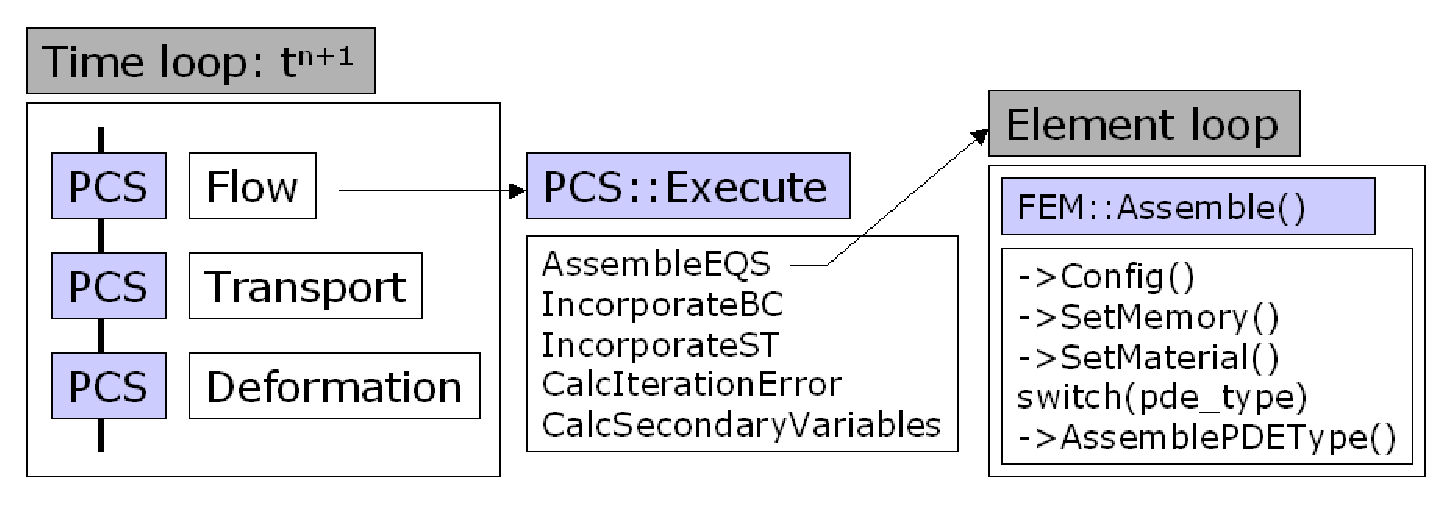
\includegraphics[scale=0.45]{figures/algorithm.eps}
\caption{Implementation of solution algorithm} \label{fig:alg}
\end{figure}

%---
\subsection{Process (PCS) types}
\label{sec:pcs}

The central idea behind object-orientation of processes is that the
basic steps of the solution procedure: calculation of element
contributions, assembly of equation system (including treatment of
boundary conditions and source terms), solution of the equations
system, linearization methods and calculation of secondary variables, 
are independent of the specific problem (e.g. flow,
transport, deformation processes) \cite{{KolBau:04},{geosys}}. The
process (PCS) class provides basic methods in order to solve a PDE
in a very general way. The central part of the PCS object is the
member function \texttt{PCS::Execute()} (Fig. \ref{fig:alg}, middle
box) conducting these basic steps. Specific properties of the
mechanical problem, such as PDE type, primary and secondary
variables and material functions, are assigned during process
configuration (member function \texttt{PCS::Config()}). In order to
configure PCS instances we take advantage of polymorphism.

Fig. \ref{fig:pcs} illustrates the object-orientation of PCS types 
for the solution of IBVPs. The PCS object was designed to manage the 
complete solution algorithm in order to build the global equation 
system (EQS). In fact, the PCS object 'only' administrates 
references to geometric (GEO) objects (points, polylines, surfaces, 
volumes); MSH objects (mesh nodes, elements and mesh topology), 
node-related data such as initial (IC) and boundary (BC) conditions 
as well as source terms (ST); material data of porous media (fluid 
(MFP), solid (MSP), medium (MMP) and chemical (MCP) properties); 
parameters of the different numerical methods (NUM). PCS instances 
have 'only' pointers to the related objects as members. \rev{Objects 
IC, BC and ST have pointers to object GEO to specify geometrical 
entities, which are managed by PCS to find element nodes on them. 
The values in IC and BC and ST are assigned to element nodes found 
be their GEO members. Object GEO also play a key role in the  
 pre/post-process of the data of the finite element method.}

\begin{figure}[htb!]
\centering
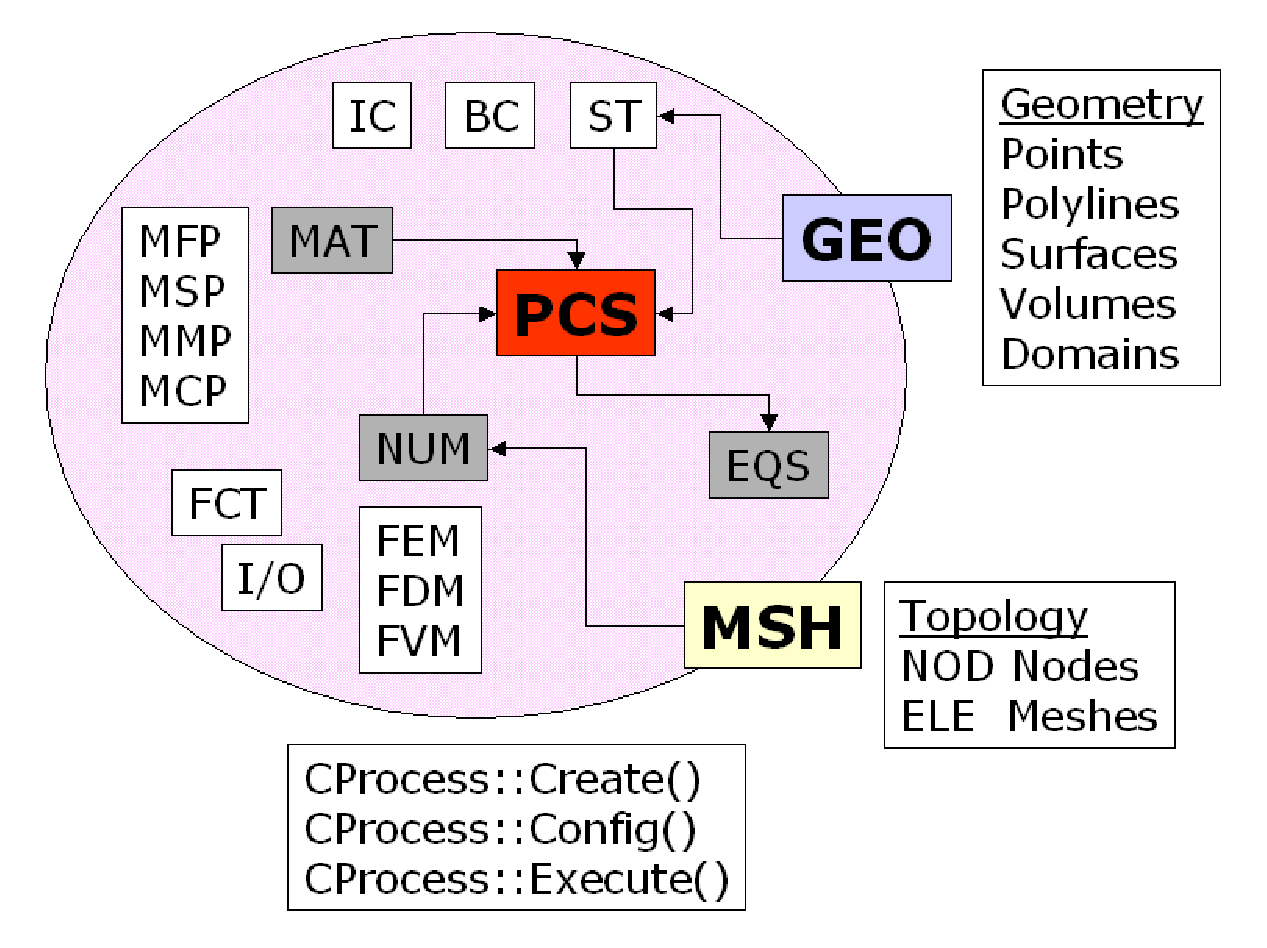
\includegraphics[scale=0.5]{figures/pcs.eps}
\caption{Structure of the process (PCS) object} \label{fig:pcs}
\end{figure}

%-------------------------------------------------------------------------
\subsection{PDE types}
\label{sec:pde}

IBVPs in porous media mechanics, such as fluid flow, mass and heat 
transport, deformation can be categorized into elliptic, parabolic, 
hyperbolic or mixed equation types.

As an example to explain the generalization of PDE types, we
illustrate the treatment of Laplace terms, which appear in flow,
transport as well as deformation processes. In Fig. \ref{fig:lap}
the evaluation of finite element matrices for Laplace terms, i.e.
$\mathbb{D}\partial^2/\partial x^2$ is given, where $\mathbb{D}$ is 
a problem-specific material tensor. The special part of diffusion 
terms is the calculation of second order space derivatives. The 
second line of the equation in Fig. \ref{fig:lap} represents the 
  numerical integration of matrix being transformated into reference coordinates. From the view point of 
object-orientation we are faced with the following operations: 
tensor coordinate transformation ($\mathbf{T}$), Jacobian 
($\mathbf{J}$), integration ($\int$) and computation of material 
properties ($\mathbb D$, e.g. diffusivity, conductivity tensor). The latter is the only problem-specific.

\begin{eqnarray}
\mathbf K_e 
&=&
\int\limits_{\Omega_e} \nabla \Sh \mathbb{D}(\nabla\Sh)^{\mathrm{T}} d\Omega \\
&=& 
\sum\limits_{gp=1}\limits^{no\_gp} \int\limits_{\Omega_r} w_{gp} 
\left[
\nabla \Sh \mathbb{D}(\nabla \Sh)^{\mathrm{T}} \mathrm{det}\ \mathbf{J} 
\right]
\vert_{gp} d\Omega
\end{eqnarray}

\begin{figure}[htb!]
\centering
\shadowbox{
\begin{minipage}{0.95\textwidth}
%{\sffamily \raggedright \small
{\ttfamily \raggedright \small
void\ CFiniteElement::CalcLaplace()\\
\{\\
\ \ \textsl{//\ Loop\ over\ Gauss\ points}\\
\ \ \textbf{for}\ (gp\ =\ 0;\ gp\ $<${}\ no\_gp;\ gp++)\\
\ \ \{\\
\mbox{\ \ \ \ \ GaussData();\ \ \ \ \ \ \ \ \ \ \ \ \ \ \ \ \ \textsl{//\ Integration\ points\ and\ weights}}\\
\mbox{\ \ \ \ \ Jacobian();\ \ \ \ \ \ \ \ \ \ \ \  \ \ \ \ \ \ \textsl{//\ det\ $\mathbf{J}$,\ ${\mathbf J}^{-1}$}}\\
\ \ \ \ \ GradShapefct();\ \ \ \ \ \  \ \ \ \ \ \ \ \ \textsl{//\ $\nabla \Sh$}\\
\mbox{\ \ \ \ \ LaplaceMATFunction();\ \ \ \ \ \ \ \ \textsl{//\ Material\ parameters,\ $\mathbb{D}$}}\\
\mbox{\ \ \ \ \ \textbf{for}\ (i=0;\ i$<${}nnodes;\ i++)\ \ \ \ \textsl{//\ Loop\ over\ element\ nodes}}\\
\ \ \ \ \ \ \ \ \textbf{for}\ (j\ =\ 0;\ j\ $<${}\ nnodes;\ j++)\\
\ \ \ \ \ \ \ \ \ \{\\
\mbox{\ \ \ \ \ \ \ \ \ \ \ \ \textbf{if}(j$>${}i)\ \textbf{continue};\ \ \ \ \textsl{//\ Symmetry}}\\
\mbox{\ \ \ \ \ \ \ \ \ \ \ \ \textbf{for}\ (k\ =\ 0;\ k\ <{}\ ele\underline\ dim;\ k++)}\\
\mbox{\ \ \ \ \ \ \ \ \ \ \ \ \ \ \ \textbf{for}(l=0;\ l<{}ele\underline\ dim;\ l++)}\\
\mbox{\ \ \ \ \ \ \ \ \ \ \ \ \ \ \ \ \ \ ($\ast$Laplace)(i,j)\ +=\ fkt\ $\ast$\ dshapefct[k$\ast$nnodes+i]\ }\\
\mbox{\ \ \ \ \ \ \ \ \ \ \ \ \ \ \ \ \ \ \ \ \ \ \ \ \ \ \ \ \ \ \ \ \ \ \ \ $\ast$\ mat[ele\underline\ dim$\ast$k+l]\ }\\
\mbox{\ \ \ \ \ \ \ \ \ \ \ \ \ \ \ \ \ \ \ \ \ \ \ \ \ \ \ \ \ \ \ \ \ \ \ \ $\ast$\ dshapefct[l$\ast$nnodes+j];}\\
\ \ \ \ \ \ \ \ \ \}\\
\ \ \}\\
\}\\
\ \\
 }
\normalfont\normalsize


\end{minipage}
}
\caption{Finite element Laplace matrix and implementation}
\label{fig:lap}
\end{figure}

\begin{figure}[htb!]
\centering
\shadowbox{
\begin{minipage}{0.75\textwidth}
{\ttfamily \raggedright \small
void\ CFiniteElementPCS::LaplaceMATFunction()\\
\{\\
\ \ \textsl{//\ Calculate\ conductivity\ tensor\ $\mathbb D$ for\ Laplacian}\\
\ \ \ \textbf{switch}(PcsType)\{\\
\ \ \ \ \ \ \textbf{case}\ L:\ \textsl{//\ Liquid\ flow}\\
\ \ \ \ \ \ \textbf{case}\ U:\ \textsl{//\ Unconfined\ flow}\\
\ \ \ \ \ \ \textbf{case}\ G:\ \textsl{//\ Gas\ flow}\\
\ \ \ \ \ \ \textbf{case}\ T:\ \textsl{//\ Two-{}phase\ flow}\\
\ \ \ \ \ \ \textbf{case}\ C:\ \textsl{//\ Componental\ flow}\\
\ \ \ \ \ \ \textbf{case}\ H:\ \textsl{//\ Heat\ transport}\\
\ \ \ \ \ \ \textbf{case}\ M:\ \textsl{//\ Mass\ transport}\\
\ \ \ \ \ \ \textbf{case}\ O:\ \textsl{//\ Overland\ flow}\\
\ \ \ \ \ \ \textbf{case}\ R:\ \textsl{//\ Richard\ flow}\\
\ \ \ \}\\
\}\\
\ \\
 }
\normalfont\normalsize


\end{minipage}
}
\caption{Implementation of process dependent material functions}
\label{fig:mat1}
\end{figure}

Fig. \ref{fig:lap} shows the implementation of the Laplace term
calculation, in which $\Omega_r$ is the domain by the reference 
element. The \texttt{CalcLaplace()} member function of the finite 
element class works for different processes with different material 
functions (Fig. \ref{fig:mat1}) and geometric element types. A short 
description is given in the table below.

\small
\begin{tabular}{|l|l|}
  \hline
  % after \\: \hline or \cline{col1-col2} \cline{col3-col4} ...
  \texttt{Code} & Description \\
  \hline
  \texttt{gp} & Gauss integration points \\
  \texttt{GaussData()} & Calculation of Gauss weights \\
  \texttt{Jacobian()} & Calculation of Jacobian determinant and inverse \\
  \texttt{GradShapeFunction()} & Calculation of shape function derivatives \\
  \texttt{LaplaceMATFunction()} & Calculation of material coefficients \\
  \texttt{(*Laplace)(i,j)} & Finite element matrix \\
  \hline
\end{tabular}
\normalsize

%-------------------------------------------------------------------------
\subsection{Element (ELE) types}
\label{sec:ele}

The basic concept we apply is that: element data, such as geometrical and topological
properties, as well as operations of elements, such as
element matrix calculations and treatment of boundary conditions,
can be generalized.

The element object is the fundamental entity in both PDE and
element types. In Fig. \ref{fig:ele_concept} the structure of the
element object is illustrated. The element has two kinds of
properties connected geometry and PDE types.

\begin{figure}[H]
\centering
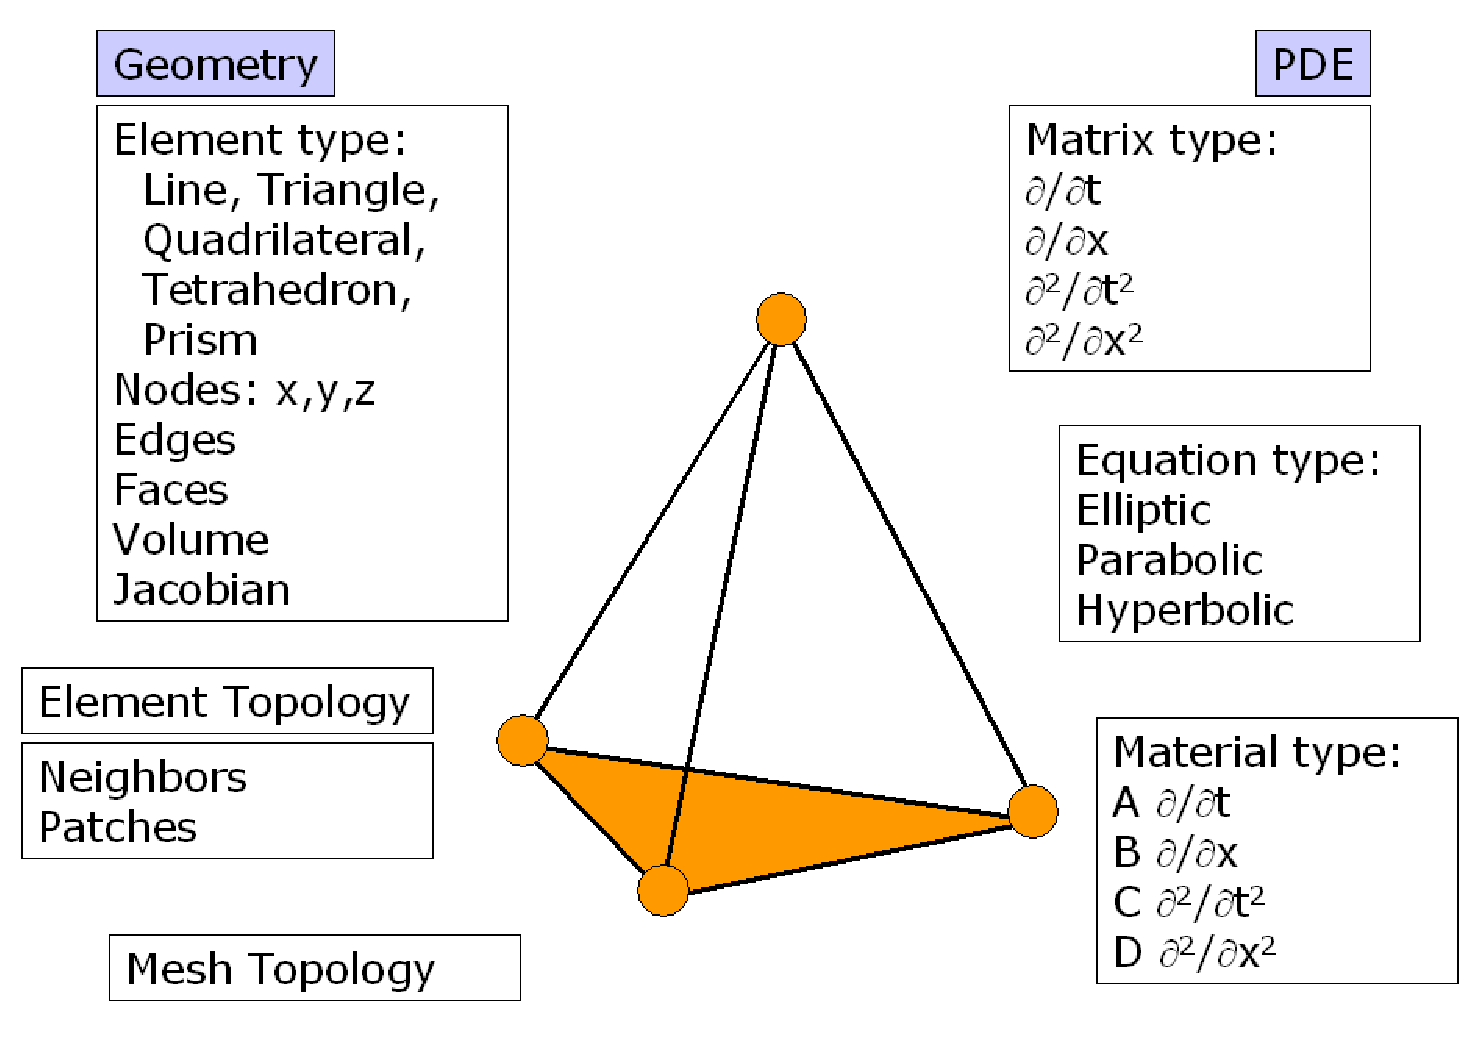
\includegraphics[scale=0.4]{figures/ele_concept.eps}
\caption{Structure of element object}
\label{fig:ele_concept}
\end{figure}

Element geometry includes the geometric type (line, triangle, quad, 
tetrahedron, prism, hexahedron), node coordinates, edges, faces and 
volume. Coordinate transformation functionalities are considered as 
geometric element properties. Element topology is defined by element 
neighbor relationships. Patch properties are available for finite 
volume approaches and flux calculations. The elements form the mesh 
topology. Different geometric element types can be combined (Fig. 
\ref{fig:ele_concept}) together to establish a mesh. Additionally, 
elements can be assigned to different meshes.
%%%% \cite{Kol:2005b}.

Depending on PDE type (elliptic, parabolic, hyperbolic, mixed),
different first or second order differential terms have to be
evaluated ($\partial/\partial t, \partial/\partial x,
\partial^2/\partial t^2, \partial^2/\partial x^2$). These differential
terms are categorized in corresponding FE matrix types (see section 
\ref{sec:fem}), mass matrix, Laplacian matrix, tangential matrix and 
coupling matrices. An obvious advantage of this element concept is 
that, depending on the geometric element type, interpolations (shape 
functions) and derivations as well as tensor operations and Gaussian 
integrations are conducted automatically in a correct way (see 
section \ref{sec:ele_fem}). For material tensor properties in 1D, 2D 
or 3D ($\mathbf{A,B,C,D(x)}$ in Fig. \ref{fig:ele_concept}), the 
correct matrix multiplications are conducted automatically. Material 
functions ($A,B,C,D(u)$ in Fig. \ref{fig:ele_concept}) are evaluated 
accordingly at corresponding Gaussian points of the selected 
element.

For the sake of object-orientation for numerical methods a so-called 
process (PCS) object was designed, implemented (\cite{KolBau:04}, 
section \ref{sec:pcs}) and successfully applied to different 
numerical methods (FEM: \cite{KolEtAl:2004a}, FDM: 
\cite{KolEtAl:2005a}, FVM: \cite{Bei:2005}).

%\providecommand{\sembrack}[1]{[\![#1]\!]}
\providecommand{\pD}[2]{\dfrac{\partial #1}{\partial #2}}
\providecommand{\oD}[2]{\dfrac{\mathrm d #1}{\mathrm d  #2}}
\providecommand{\abs}[1]{\lvert #1 \rvert}
%%\providecommand{\abs}[1]{\left\lvert #1 \right\rvert}
\providecommand{\norm}[1]{\left\lVert #1 \right\rVert}

\newcommand{\od}{\mathrm d}
%%%
\newcommand{\js}{\mathscr S}
%%%
%%material index
\newcommand{\pl}{\scriptscriptstyle \mathrm p}
\newcommand{\el}{\scriptscriptstyle \mathrm e}

%%Geometry
\newcommand{\Point}{ \bm x}

%%Displacement field
\newcommand{\Pressure}{p}
\newcommand{\Stress}{ \bm \sigma}
\newcommand{\inPStress}{ \Stress_{\imath}} %%% in-plane stress
\newcommand{\stress}{ \sigma}
\newcommand{\devStrs}{\bm s}
\newcommand{\Strain}{ \bm \epsilon}
\newcommand{\strain}{ \epsilon}
\newcommand{\Disp}{\mathbf u}
\newcommand{\disp}{u}
\newcommand{\vel}{\bf v}
\newcommand{\per}{\mathbf k}
\newcommand{\grv}{\mathbf g}
%%Plasticity
\newcommand{\yld}{ f}
\newcommand{\ppo}{ g}
\newcommand{\pHard}{\mathcal H}
\newcommand{\CT}{\mathbb C}
\newcommand{\DT}{\mathbb D}
\newcommand{\EM}{{\bm C}^{\el}}
\newcommand{\PM}{{\bm C}^{\pl}}
\newcommand{\EPM}{{\bm C}^{\el\pl}}
\newcommand{\mEM}{{\bm D}^{\el}}
\newcommand{\mPM}{{\bm D}^{\pl}}
\newcommand{\mEPM}{{\bm D}^{\el\pl}}
\newcommand{\rdl}{\dot \lambda}
\newcommand{\dl}{\lambda}
\newcommand{\dens}{\rho}

%%Flow
\newcommand{\densc}{\dens^{\gamma}}
\newcommand{\presc}{p^{\gamma}}
\newcommand{\pres}{p}
\newcommand{\sat}{S}
\newcommand{\Satc}{S^{\gamma}}
\newcommand{\RelK}{k^{\gamma}_{rel}}
\newcommand{\RelKa}{k_{rel}}
\newcommand{\poro}{n}
\newcommand{\Fluxf}{\mathbf{q}_{\scriptscriptstyle f}}
\newcommand{\Fluxv}{\mathbf{q}_{\scriptscriptstyle v}}
\providecommand{\perm}{ \mathbf k}
\newcommand{\asup}[2]{#1^#2}
\newcommand{\asub}[2]{#1_#2}
\newcommand{\supsub}[3]{{#1}^{#2}_{#3}}
\newcommand{\FlxDf}{\mathbf{J}}
\newcommand{\Sat}{S}
%%Heat
\newcommand{\HC}{C_p}
\newcommand{\Flux}{\mathbf{q}}

%%%FEM
\newcommand{\test}{w}
\newcommand{\Test}{\bm w}
\newcommand{\TestS}{\mathcal V}
\newcommand{\sh}{N}
% \newcommand{\Sh}{{\bm N}}

%%Math
\newcommand{\intD}{{\int}_{\Omega}}
\newcommand{\intB}{{\int}_{\Gamma}}
\newcommand{\dDom}{\,\mathrm{d} \Omega}
\newcommand{\dBdry}{\,\mathrm{d} \Gamma}
\newcommand{\nrl}{\mathbf n}
\newcommand{\tgl}{\mathbf t}
\newcommand{\I}{\mathbf I}

\section{General finite element formulations}
\label{sec:fem}

The method of weighted residuals is applied to derive the weak
formulation of the balance equations given in section
\ref{sec:balance_equations}.

Assume $\TestS^{\mathrm{n}}\subset
H^1_{\scriptscriptstyle{\Gamma}}(\Omega)^{\mathrm{n}}$ is the test
function space. For all $\test\in \TestS^{\mathrm{1}}$, we have
the weak form of the mass balance equation (\ref{eqn:phase_mass_balance}) as
%
\begin{gather}
\int_\Omega 
\left(
nS^{\gamma} \frac{\partial\rho^{\gamma R}}{\partial t} + nS^{\gamma} \mio{v}{\gamma s}{} \cdot \nabla \rho^{\gamma R}
+
n\rho^{\gamma R}\frac{\partial S^{\gamma}}{\partial t} + n\rho^{\gamma R} \mio{v}{\gamma s}{} \cdot \nabla S^{\gamma}
\nonumber  %[1.5ex]
+
\nabla \cdot
(\rho^{\gamma}nS^{\gamma} \mio{v}{\gamma s}{} )
+S^{\gamma}\rho^{\gamma R}\nabla\cdot\mio{u}{s}{\dot} 
- q^{\gamma}
\right)
\test\dDom = 0
\label{eq:wkmass0}
\end{gather}
%
Applying integration by parts, divergence terms can be rewritten as
%
\begin{gather}
\int_\Omega \nabla\cdot\mio{A}{}{} \omega d\Omega
=
\int_\Omega \mio{A}{}{} \cdot \nabla\omega \dDom
+
\int_\Gamma \mio{A}{}{} \cdot \mathbf{n} \omega \dBdry
\label{eq:wkmass}
\end{gather}

Under the same assumption, the weak form of heat balance equation (\ref{eqn:energy_balance}) can be obtained as
\begin{gather}
\int_\Omega \sum_{\gamma}(\varepsilon^\alpha\rho^\alpha c_p^\alpha)\pD{T}{t}\test\dDom
-
\int_\Omega \miu{j}{\mathrm{th}}{} \cdot \nabla\omega \dDom
+
\int_\Gamma \miu{j}{\mathrm{th}}{} \cdot \mathbf{n} \omega \dBdry
-
\intD Q_{\mbox{\tiny T}}^{\gamma}\test\dDom=0
\label{eq:wkhTmass}
\end{gather}

Taking account of nonlinearity, the weak form of the momentum balance equation
(\ref{eq:4}) must be fulfilled throughout the load history, i.e.,
%
\begin{equation}
\intD \frac{1}{2}(\miu{\sigma}{\mathrm{eff}}{} - \sum_\gamma\sat^\gamma p^\gamma \I ):(\nabla \Test+(\nabla \Test)^{\mathrm T}) \dDom 
-
\intD\Test^{\mathrm T} \cdot \dens \grv \dDom  - \intB
\Test^{\mathrm T} \cdot {\mathbf{t}} \dBdry = 0 \label{eq:wkstress}
\end{equation}
for all $\Test\in \TestS^{\mathrm{n}}, \, \mathrm{n}=2,3$.
In principle, vector form of stress and strain tensor (cf. section \ref{sec:m_properties})
are used to developing  the system equation of the discretized form of (\ref{eq:wkstress}). Under this form,
 the constitutive law for the effective stress tensor can be expressed as
\[
    \miu{\sigma}{\mathrm{eff}}{} = \miu{C}{}{}\, \miu{\varepsilon}{}{}
\]
with the corresponding strain-displacement relationship
\[
    \miu{\varepsilon}{}{} = \mathcal{L} \,\mio{u}{s}{}
\]
where $\mathcal{L}$ is an differential operator.

\begin{equation}
\mathcal{L} =
\left(%
\begin{array}{ccc}
 \partial/\partial x & 0 & 0 \\
 0 & \partial/\partial y & 0 \\
 0 & 0 & \partial/\partial z \\
 \partial/\partial y & \partial/\partial x & 0 \\
 0 & \partial/\partial z & \partial/\partial y \\
 \partial/\partial z & 0 & \partial/\partial x
\end{array}%
\right)
\label{eqn:diffop}
\end{equation}

We use the Galerkin finite element method to solve the weak forms of
balance equations above. All variables are approximated by
admissible finite element functions in the Taylor-Hood finite
element space, i.e, low order interpolation $\Sh_1\in
\mathbb{R}^{\mathrm{n}}$ for pressure and temperature variables and
high order interpolation $\Sh_2 \in \mathbb{R}^{\mathrm{n}}$ for
displacement, respectively. As a result of the finite element
discretization of the weak forms (\ref{eq:wkmass}),
(\ref{eq:wkhTmass}) and (\ref{eq:wkstress}), we obtain local
matrices and vectors for the global system equations
\cite{Kol:02}. Element matrices and vectors can be classified
into following types (Table \ref{tab:types})

\begin{table}[H]
\centering
\begin{tabular}{lll}
\hline
Type & Name & Equations
\\
%-------------------------------------------------------------------------
\hline
$ \intD \Sh_1^{\mathrm{T}} \mathcal{M} \Sh_1 \dDom $ %\label{eq:massM} $
& Mass matrix
& (\ref{eq:wkmass}),(\ref{eq:wkhTmass})
\\
%-------------------------------------------------------------------------
$ \intD (\Sh_1)^{\mathrm{T}} \mathcal{M} \nabla \Sh_1 \dDom $ %\label{eq:LapM} $
& Advection matrix
& (\ref{eq:wkhTmass})
\\
%-------------------------------------------------------------------------
$ \intD (\nabla \Sh_1)^{\mathrm{T}} \mathcal{M} \nabla \Sh_1 \dDom $ %\label{eq:LapM1} $
& Laplace matrix
& (\ref{eq:wkmass}),(\ref{eq:wkhTmass})
\\
%-------------------------------------------------------------------------
$ \intD \mathbf B^{\mathrm{T}} \mathcal{M}  \mathbf B \dDom $ %\label{eq:Tang} $
& Tangential matrix
& (\ref{eq:wkstress})
\\
%-------------------------------------------------------------------------
$ \intD \mathcal{M} {\mathbf B}^{\mathrm{T}} \mathbf{m} \Sh_1 \dDom $ %\label{eq:CDMatrix} $
& Displacement coupling matrix
& (\ref{eq:wkmass})
\\
%-------------------------------------------------------------------------
$ \intD \mathcal{M}\Sh_1^{\mathrm{T}} \mathbf{m}^{\mathrm{T}} \mathbf B\dDom $ %\label{eq:CMatrix} $
& Pressure coupling matrix
& (\ref{eq:wkstress})
\\
%-------------------------------------------------------------------------
$ \intD Q \Sh_1 \dDom \quad \mbox{,} \,\intD Q \Sh_2 \dDom $ %\label{eq:SourceV} $
& Source term vector
& (\ref{eq:wkmass}),(\ref{eq:wkhTmass}),(\ref{eq:wkstress})
\\
%-------------------------------------------------------------------------
$ \intB q \Sh^{\scriptscriptstyle \Gamma} \dBdry $ %\label{eq:NeuV} $
& Neumann vector
& (\ref{eq:wkmass}),(\ref{eq:wkhTmass}),(\ref{eq:wkstress})
\\
%-------------------------------------------------------------------------
\hline
\end{tabular}
\caption{Matrix and vector types} \label{tab:types}
\end{table}

where $\mathcal{M}$ are a process-specific material functions,
$\mathbf B= \mathcal L \Sh_2$ is so called strain-displacement
matrix, $\mathbf m = (1,\,1,\,1,\,0,\,0,\,0)^T$ is mapping vector. Based on
this classification of matrix and vector types the finite element
object is designed (section \ref{sec:ele_fem}).

\section{Element objects - ELE}

In this section, the details of the implementation of the element 
objects are described. The relationship of element objects is shown 
in Fig. \ref{fig:ele_objects}. For the simulation of each process in 
a coupled problem or each single problem, only an instance of  mesh 
object (ELE-MSH) and an instance of finite element object are 
required. Geometric element object (ELE-GEO) manufacture the 
foundation of this concept (section \ref{sec:ele_geo}). Meshes 
(ELE-MSH) are formed based from geometric element entities (section 
\ref{sec:ele_msh}). Finite element object (ELE-FEM) basically 
compute the finite element matrices for different PDE types and 
geometric element types automatically  using the corresponding shape 
functions (section \ref{sec:ele_fem}).  ELE-PCS object assemble the 
equation systems for the problem type, i.e. THM coupled ELE-PCS 
object problems for porous media (section \ref{sec:ele_pcs}). 
\rev{To this purpose, objects  ELE-PCS and ELE-FEM and have a 
pointer member pointing to each other. When an instance of ELE-PCS 
object for a process in a coupled problem or a single problem is 
constructed, an instance of ELE-FEM object is created accordingly. 
During the construction of the instance of ELE-FEM object, the 
degree of freedom of the problem is initialized by the type the 
ELE-PCS instance, i.e. the specific problem. This means only one 
instance of ELE-PCS and one instance of ELE-FEM  have to been 
created for each process in a coupled problems or for each single 
problem. Moreover, ELE-FEM has a pointer member pointing to 
interpolation function. This member is initialized by the messages 
from the instance of ELE-PCS and each instance of ELE-GEO for each 
finite element during the local assembly. Such initialization 
guarantees that interpolation function and its derivatives are set 
properly for each geometric element for a process or a problem. 

\begin{figure}[!htb]
\centering
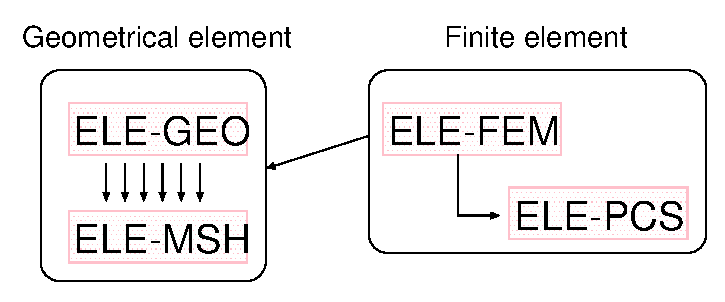
\includegraphics[scale=0.8]{figures/ele_relation.eps}
\caption{Relationship of element objects} 
\label{fig:ele_objects}
\end{figure}

In general, messages of the type of a process a problem and the type 
element determines the pointers to the corresponding interpolation 
function and its derivatives of an instance of ELE-FEM.   An 
instance of ELE-FEM has a pointer to  ELE-GEO as a member too. When 
local assembly comes to an element, or an instance of ELE-GEO, the 
ELE-FEM instance have the ELE-GEO pointer point to the element and 
initialized its numerical methods such as interpolation, Guass 
integration accordingly. This is very helpful for the finite element 
analysis of consolidation in porous media, in which, the Talyor-Hood 
finite element spaces, i.e. linear interpolation for flow process 
and quadratic interpolation for deformation process, is required for 
stability reason\cite{LeSch:98}. In default, the order of 
interpolation of each element is linear and the nodes of an element 
are its geometrical vertices.  If the high order interpolation is 
required by a process or a problem, additional nodes are created for 
each instance of ELE-FEM during the construction of the mesh.} The 
idea of this concept is, that specific process-related information 
are introduced as late as possible to keep the software concept as 
flexible as possible.

\subsection{Geometric element object -- ELE-GEO}
\label{sec:ele_geo}

As described in section \ref{sec:ovl}, the first step of finite
element analysis is the domain discretization. As a result we
obtain element meshes. Hereafter, we refer to a mesh element as
the geometric element object \texttt{ELE-GEO}. The intrinsic
properties of a geometric element object are: nodes, edges, faces, volume and neighbors (Fig. \ref{fig:elem}). Neighbor relationships connect
geometric element objects within a mesh and, therefore, represent
topological properties.

\begin{figure}[H]
\centering
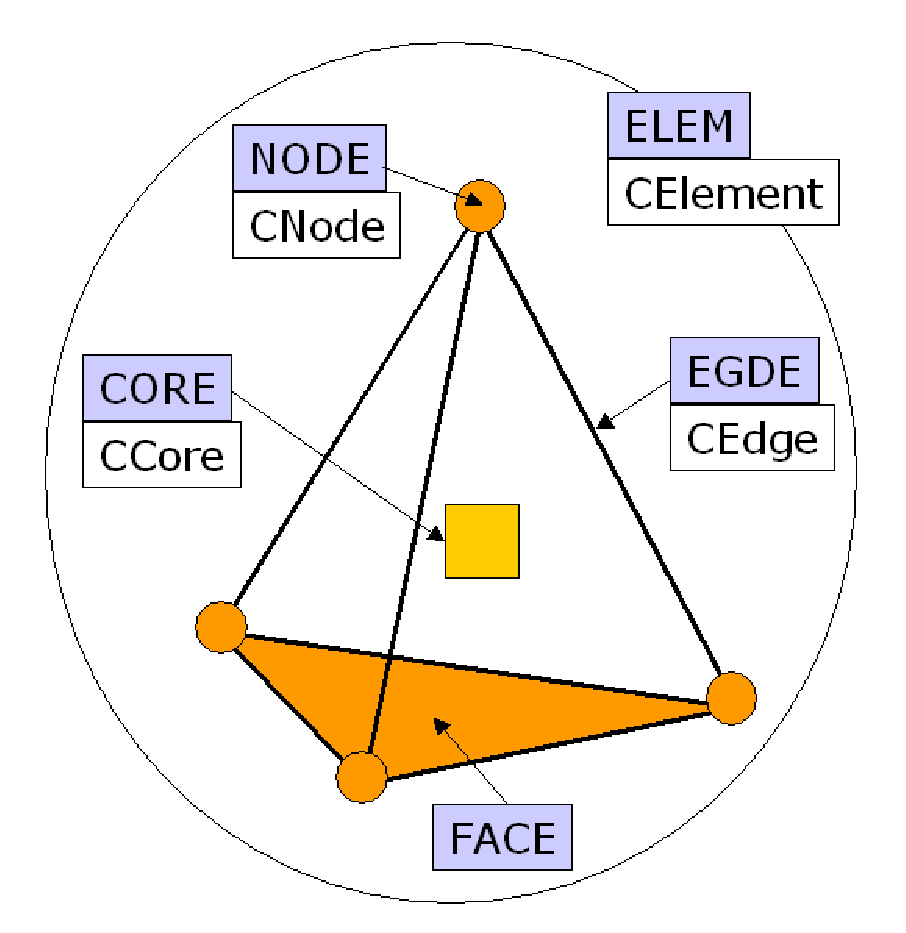
\includegraphics[scale=0.4]{figures/elem.eps}
\caption{Mesh element}
\label{fig:elem}
\end{figure}

%\begin{figure}[H]
%\centering
%\includegraphics[scale=0.7]{figure/gelement}
%\caption{Geometric element properties}
%\label{fig:gele}
%\end{figure}

We design the following element property classes to encapsulate
all geometric and topological element information.

\begin{itemize}
  \item \texttt{CCore} for \texttt{CORE} object,
  \item \texttt{CNode} for \texttt{NODE} object,
  \item \texttt{CEdge} for \texttt{EDGE} object,
  \item \texttt{CElem} for \texttt{ELEM} object.
\end{itemize}

Faces and neighbors belong to \texttt{ELEM} object. Indeed, edges
could be also assigned to the \texttt{ELEM} object. However, we
consider an edge as an individual entity for two reasons. First,
some numerical methods, such as mixed finite elements, require edges
as a basic geometric property as nodes for the Galerkin FEM. Second,
edges are frequently used as basic properties \rev{in automatic
generation}. As \texttt{NODE}, \texttt{EDGE} and \texttt{ELEM}
objects share common data and methods, we abstract these into the
\texttt{CCore} class as a base class.

\begin{figure}[H]
\centering
\shadowbox{
\begin{minipage}{0.9\textwidth}
{
\ttfamily \raggedright \small
\texttt{class\ CCore\\
\{\\
\ \ \ \textbf{protected}: // Properties\\
\ \ \ \ \ \ \textbf{long}\ index; // global element index\\
\ \ \ \ \ \ \textbf{char}\ position; // position indicator\\
%\ \ \ \ \ \ \textsl{//\ Status\ in\ usage}\\
\ \ \ \ \ \ \textbf{bool}\ status; //\ status\ in\ usage \\
%\ \ \ \ \ \ \textsl{//\ High\ order}\\
\ \ \ \ \ \ \textbf{int}\ order; // order of interpolation\\
\ \ \ \textbf{public}: // Methods\\
\ \ \ \ \ \ \textsl{//\ Set\ members}\\
\ \ \ \ \ \ \textbf{void}\ SetIndex(\textbf{const}\ \textbf{long}\ index)\ \{index\ =\ index;\}\\
\ \ \ \ \ \ \textbf{void}\ SetPosition(\textbf{const}\ \textbf{char}\ BC\underline\ type)\ \{boundary\ =\ BC\underline\ type;\}\\
\ \ \ \ \ \ \textbf{void}\ SetStatus(\textbf{const}\ \textbf{bool}\ status)\ \{status\ =\ status;\}\\
\ \ \ \ \ \ \textbf{void}\ SetOrder(\textbf{const}\ \textbf{int}\ order)\ \{order\ =\ order;\}\\
\ \ \ \ \ \ \textsl{//\ Get\ members}\\
\ \ \ \ \ \ \textbf{long}\ GetIndex()\ \textbf{const}\ \{\textbf{return}\ index;\}\ \\
\ \ \ \ \ \ \textbf{char}\ GetPosition()\ \textbf{const}\ \{\textbf{return}\ position;\}\ \\
\ \ \ \ \ \ \textbf{bool}\ GetStatus()\ \textbf{const}\ \{\textbf{return}\ status;\}\\
\ \ \ \ \ \ \textbf{int}\  GetOrder()\ \textbf{const}\ \{\textbf{return}\ order;\}\\
\ \ \ \ \ \ \textsl{//\ Construction}\\
\ \ \ \ \ \ CCore(\textbf{const}\ \textbf{int}\ id); // constructor\\
\ \ \ \ \ \ \textbf{virtual}\ \ \textasciitilde CCore(); // destructor\\
\ \ \ \ \ \ \textsl{//\ Operators}\\
\ \ \ \ \ \ \textbf{virtual}\ \textbf{void}\ \textbf{operator}\ =\ (\textbf{const}\ CCore\ \&\ g)\ \{\}\\
\ \ \ \ \ \ \textbf{virtual}\ \textbf{bool}\ \textbf{operator}\ ==\ (\textbf{const}\ CCore\ \&\ g)\ \{\textbf{return}\ \textbf{false};\}\\
\ \ \ \ \ \ \textsl{//\ Output}\\
\ \ \ \ \ \ \textbf{virtual}\ \textbf{void}\ output(ostream\&\ os=cout)\ \textbf{const}\ \{\};\\
\};\\
}
}
\normalfont\normalsize

\end{minipage}
}
\caption{\texttt{CCore} implementation for basic geometric element properties and methods}
\label{fig:core}
\end{figure}

\vfill

\newpage
%----------------------------------------------------------------------
\subsubsection{Core object - \texttt{CORE} - geometric element base class}
\label{sec:core}

Common data of a geometric element are: global element index;
position indicator within the whole domain, which indicates whether
the geometric element is inside the domain or on the domain surface;
%with specific boundary condition type;
status flag, which indicates whether this element is marked for
some usage. Assign $=$ as well as identity operators $==$ are
virtually defined. The C++ implementation of the \texttt{CCore} base
class is given in Fig. \ref{fig:coree}.

\begin{figure}[H]
\centering
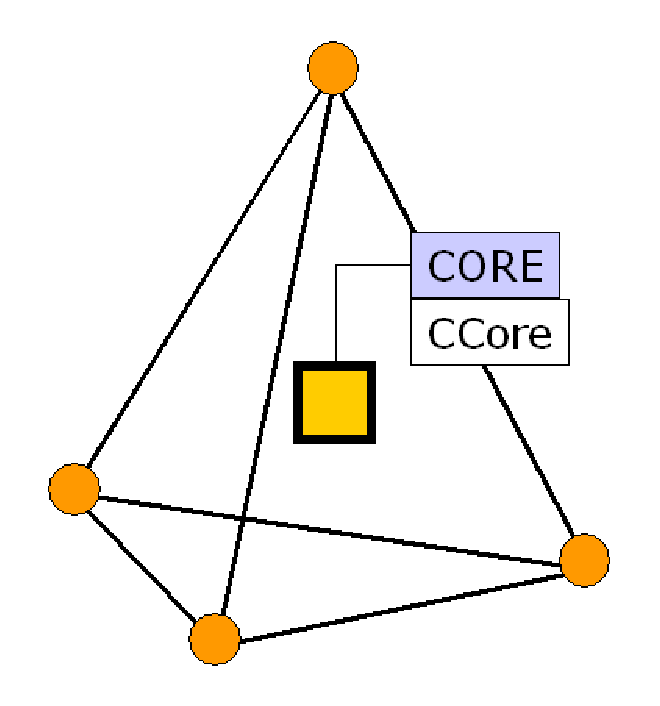
\includegraphics[scale=0.4]{figures/core.eps}
\caption{Core of mesh element} \label{fig:coree}
\end{figure}

\rev{Member \mbox{\texttt{char position}} is used to determine the
location of the geometrical entity within a domain, e.g. it is
inside the domain or on the boundary of the domain.}
%%\input{code/core}

Classes \texttt{CNode}, \texttt{CEdge} and \texttt{CElem} are
directly derived from the base class \texttt{CCore}. Assign $=$ as
well as the identity operator $==$ are overloaded in these
objects. With such overloading operators, passing data of an class
instance, \texttt{A}, to another class instance, \texttt{B}, can
be simply realized with the instruction
\mbox{\texttt{A}=\texttt{B}}. Whether two instances are identical
can be checked by the instruction
\mbox{\texttt{if}(\texttt{A}==\texttt{B})}.

\begin{figure}[H]
\centering
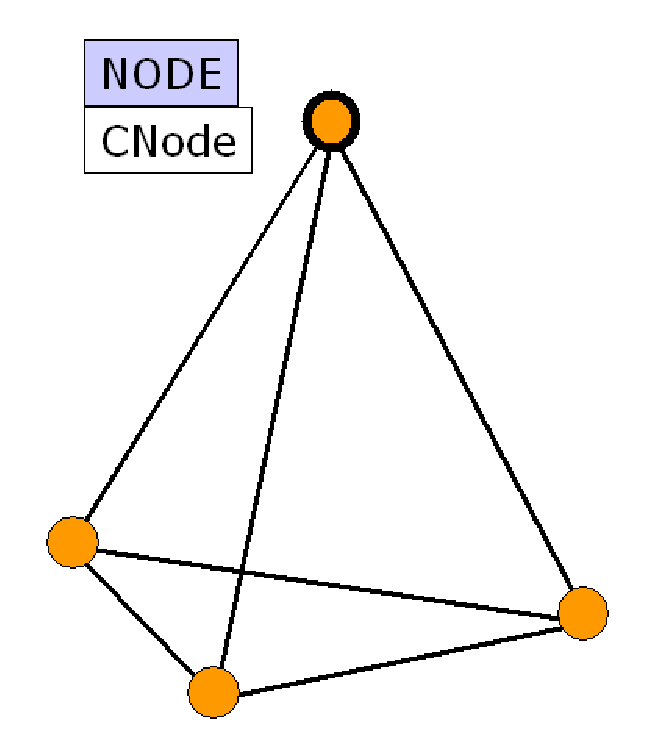
\includegraphics[scale=0.4]{figures/node.eps}
\caption{Node of element object} \label{fig:node1}
\end{figure}

%----------------------------------------------------------------------
\subsubsection{Node object - \texttt{NODE}}
\label{sec:node}

The node object (\texttt{NODE}) is derived from the \texttt{CCore}
class. In addition, the \texttt{CNode} class provides the
geometrical position of an element in real space, i.e. the coordinates
of element nodes (Fig. \ref{fig:node1}).

\begin{figure}[H]
\centering
\shadowbox{
\begin{minipage}{0.95\textwidth}
{\sffamily \raggedright
\footnotesize \texttt{class\ CNode:\textbf{public}\ CCore\\
\{\\
\ \ \ \textbf{private}: // Members\\
\ \ \ \ \ \ \textbf{double}\ coordinate[3];\\
\ \ \ \ \ \ Vector$<${}\textbf{long}$>${} ConnectedElements;\ \ \ \\
\ \ \ \ \ \ \rev{Vector$<${}\textbf{long}$>${} ConnectedNodes;}\ \ \ \\
\ \ \ \textbf{public}:\\
\ \ \ \ \ \ \textsl{//\ Construction}\\
\ \ \ \ \ \ Node(\textbf{const}\ \textbf{int}\ Index,\ \textbf{const}\ \textbf{double}\ x,\ \\
\ \ \ \ \ \ \ \ \ \ \ \textbf{const}\ \textbf{double}\ y,\ \textbf{const}\ \textbf{double}\ z=0.0);\\
\ \ \ \ \ \ Node()\ \{\}\\
\ \ \ \ \ \ \textasciitilde Node()\ \{ConnectedElements.resize(0); ConnectedNodes.resize(0);\}\\
\ \ \ \ \ \ \textsl{//\ Operators}\\
\ \ \ \ \ \ \textbf{void}\ \textbf{operator}\ =\ (\textbf{const}\ Node\&\ n);\\
\ \ \ \ \ \ \textbf{bool}\ \textbf{operator}\ ==\ (\textbf{const}\ Node\ \&\ n);\\
\ \ \ \ \ \ \textsl{//\ Set members}\\
\ \ \ \ \ \ \textbf{void}\ SetX(\textbf{const}\ \textbf{double}\ argX)\ \{\ coordinate[0]\ =\ argX;\}\\
\ \ \ \ \ \ \textbf{void}\ SetY(\textbf{const}\ \textbf{double}\ argY)\ \{\ coordinate[1]\ =\ argY;\}\\
\ \ \ \ \ \ \textbf{void}\ SetZ(\textbf{const}\ \textbf{double}\ argZ)\ \{\ coordinate[2]\ =\ argZ;\}\\
\ \ \ \ \ \ \textbf{void}\ SetCoordinates(\textbf{const}\ \textbf{double}$\ast$\ argCoord);\ \\
\ \ \ \ \ \ \textsl{//\ Get members}\\
\ \ \ \ \ \ \textbf{double}\ GetX()\ \textbf{const}\ \{\textbf{return}\ coordinate[0];\}\\
\ \ \ \ \ \ \textbf{double}\ GetY()\ \textbf{const}\ \{\textbf{return}\ coordinate[1];\}\\
\ \ \ \ \ \ \textbf{double}\ GetZ()\ \textbf{const}\ \{\textbf{return}\ coordinate[2];\}\\
%\ \ \ \ \ \ \textbf{void}\ Coordinates(\textbf{double}\ $\ast$xyz)\ \textbf{const}\\
%\ \ \ \ \ \ \{\ \ \textbf{for}(\textbf{int}\ i=0;\ i$<${}3;\ i++)\ \ xyz[i]\ =\ Coordinate[i];\}\ \\
\ \ \ \ \ \ \textbf{int}\ GetNumberOfConnectedElements()\ \textbf{const}\ \{\textbf{return}\ ConnectedElements.size();\ \}\ \ \ \ \ \\
\ \ \ \ \ \ \rev{\textbf{int}\ GetNumberOfConnectedNodes()\ \textbf{const}\ \{\textbf{return}\ ConnectedNodes.size();}\ \}\ \ \ \ \ \\
\ \ \ \ \ \ \textsl{//\ Output}\\
\ \ \ \ \ \ \textbf{void}\ Write(ostream\&\ os=cout)\ \textbf{const};\\
\ \ \ \textbf{private}: // Class relations\\
\ \ \ \ \ \ \textbf{friend}\ \textbf{class}\ CEdge;\\
\ \ \ \ \ \ \textbf{friend}\ \textbf{class}\ CElem;\\
\};\\
}
 }
\normalfont\normalsize

\end{minipage}
}
\caption{\texttt{CNode} implementation}
\label{fig:node}
\end{figure}

Mesh elements having this node in common are determined immediately
after mesh data is generated. Elements sharing this node are stored
in vector \texttt{ConnectedElements}. This node-element relationship
is very important information of the mesh topology. It is required
e.g. for extrapolation of Gauss point values to node values or for
projecting element properties to nodes. Using the
\texttt{ConnectedElements} vector, the calculation of mesh topology
can be enormously accelerated. \rev{For extrapolation of gauss point
values to nodes, we only need to know the size of the vector, i.e.
how many element connected to the nodes. Since extrapolation takes
place in element-wise, node values are accumulated from the
contribution of its connected elements, we have to average the
accumulated node value by dividing it with the number of connected
elements after extrapolation is finished. Member vector
\texttt{ConnectedNodes} stores indices of all nodes of connected
elements and it used together with the degree of freedom of the
preocess/problem to store indices of all nodes of connected elements
and it can be used together with the degree of freedom of the
preocess/problem to create the sparse matrix of the system
equations.to create the sparse matrix of the system equations. The
memory of \texttt{ConnectedNodes} is released as soon as the sparse
matrix is created.} Classes \texttt{CEdge} and \texttt{CElem} are
set as friend classes of \texttt{CNode} so that they can access to
\texttt{CNode} private members directly. The C++ implementation of
\texttt{class CNode} is given in Fig. \ref{fig:node}.

Instances of \texttt{NODE} object are stored in a global vector: \\
\texttt{vector<CNode*>node\_vector}.

%----------------------------------------------------------------------
\subsubsection{Edge object - \texttt{EDGE}}
\label{sec:edge}

The edge object (\texttt{EDGE}) is derived from the \texttt{CCore}
class. Edges are used to build up the frame of a geometric element
object (Fig. \ref{fig:gedge}). It is sufficient to use two nodes to
form a geometric edge. However, for higher order finite elements,
more points are required along an edge. Therefore, we use a vector
of \texttt{CNode} pointers as class member for edge nodes (see Fig.
\ref{fig:gedge}). In case of quadratic finite elements, the first
two nodes are element corner nodes and the last one is the middle
point of this edge.

\begin{figure}[H]
\centering
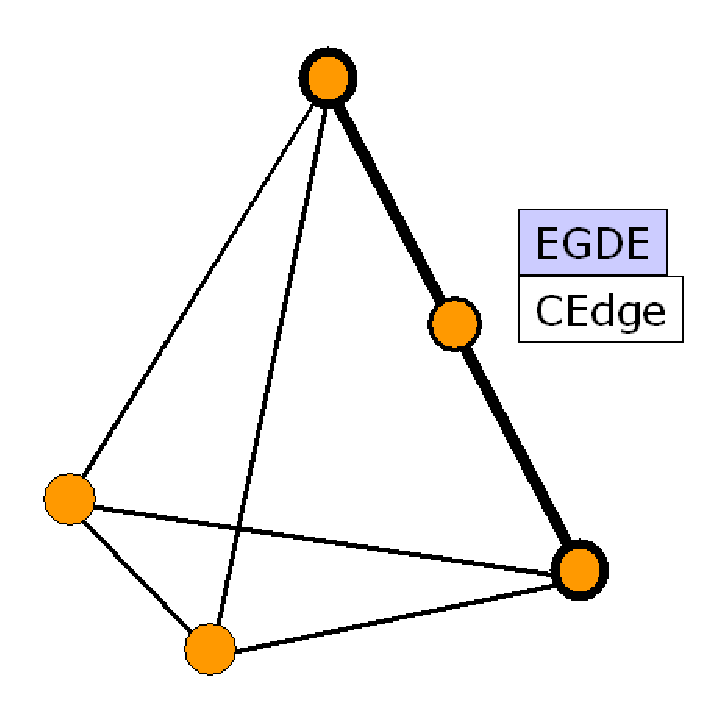
\includegraphics[scale=0.4]{figures/edge_new.eps}
\caption{Edge of mesh element} \label{fig:gedge}
\end{figure}

The C++ implementation of the \texttt{CEdge} class is given in
Fig. \ref{fig:edge}.

\texttt{Vector} is a "clone" of the standard C++ vector template,
as \texttt{template Vector\-<class V> class V} with less memory consuming but sufficient
and efficient functionality of vector algebraic calculation.

For node based finite elements (i.e. linear
interpolation), edges are only used to the compute topological mesh
structure \rev{and to process Dirichlet  boundary conditions and
source terms. For instance, if a Dirichlet  boundary condition of a
PDE is assigned by a polyline, edges of elements on the polyline
will be found and the Gauss integration will be performed on these
edges to produce node values of nodes of these edges}. They are not
needed to be stored for the later computations anymore. On the other
hand, mixed finite elements or higher order finite elements require
edges through all computations. In this case we save all edges of a
mesh in a standard C++ vector: \texttt{vector<CEdge*>egde\_vector}.

\begin{figure}[H]
\centering
\shadowbox{
\begin{minipage}{0.95\textwidth}
{
\sffamily \raggedright \scriptsize
\texttt{class\ CEdge:\textbf{public}\ CCore\\
\{\\
\ \ \ \textbf{private}: // Members\\
\ \ \ \ \ \ vec$<${}CNode$\ast>${}\ nodes\underline\ of\underline\ edges;\\
\ \ \ \textbf{public}: // Member functions\\
\ \ \ \ \ \ \textsl{//\ Construction}\\
\ \ \ \ \ \ Edge(\textbf{const}\ \textbf{int}\ Index,\ \textbf{bool}\ quadr=\textbf{false});\\
\ \ \ \ \ \ \textasciitilde Edge();\ \\
\ \ \ \ \ \ \textsl{//\ Operators}\\
\ \ \ \ \ \ \textbf{void}\ \textbf{operator}\ =\ (CEdge\&\ edg);\\
\ \ \ \ \ \ \textbf{bool}\ \textbf{operator}\ ==\ (CEdge\&\ edg);\\
\ \ \ \ \ \ \textsl{//\ Member access}\\
\ \ \ \ \ \ \textbf{void}\ SetNodes(\ vec$<${}CNode$\ast>${}\&\ Nodes)\\
\ \ \ \ \ \ \{\ \textbf{for}(\textbf{int}\ i=0;\ i$<${}(\textbf{int})Nodes.Size();\ i++)\ \ Nodes[i]\ =\ nodes\underline\ of\underline\ edges[i];\ \}\\
\ \ \ \ \ \ \textbf{void}\ SetNodes(\ vec$<${}CNode$\ast>${}\&\ Nodes)\ \textbf{const}\ \{\ Nodes\ =\ nodes\underline\ of\underline\ edges;\}\\
\ \ \ \ \ \ \textsl{//\ Output}\\
\ \ \ \ \ \ \textbf{void}\ Write(ostream\&\ osm=cout)\ \textbf{const};\\
\ \ \ \textbf{private}: // Class relations\\
\ \ \ \ \ \ Vector$<${}CNode$\ast>${}\ \ nodes\underline\ of\underline\ edges;\\
\ \ \ \ \ \ \textbf{friend}\ \textbf{class}\ CElem;\\
\};\\
}
 }
\normalfont\normalsize

\end{minipage}
}
\caption{\texttt{CEdge} implementation}
\label{fig:edge}
\end{figure}

%
\begin{figure}[H]
\centering
\shadowbox{
\begin{minipage}{0.9\textwidth}
{
\sffamily \raggedright \scriptsize
\texttt{class\ CElement:\textbf{public}\ CCore\\
\{\\
\ \ \ \textbf{private}:\ \textsl{//\ Members}\\
\ \ \ \ \ \ \textsl{//\ ID}\\
\ \ \ \ \ \ CElem$\ast$\ owner;\\
\ \ \ \ \ \ \textbf{int}\ ele\underline\ type;\ \ \textsl{//\ Element\ type}\\
\ \ \ \ \ \ \textsl{//\ Geometrical properties}\\
\ \ \ \ \ \ \textbf{int}\ dim;\ \ \ \ \ \ \ \textsl{//\ dimension\ of\ element}\\
\ \ \ \ \ \ \textbf{double}\ volume;\ \textsl{// element volume}\\
\ \ \ \ \ \ \textsl{//\ Topological properties}\\
\ \ \ \ \ \ \textbf{int}\ nnodes;\ \ \ \ \textsl{//\ number\ of element corner nodes}\\
\ \ \ \ \ \ \textbf{int}\ nnodesHQ;\ \ \textsl{//\ number of element nodes for quadratic interpolation}\\
\ \ \ \ \ \ Vector$<${}CNode$\ast>${}\ \ nodes;\\
\ \ \ \ \ \ \textbf{int}\ nedges;\ \ \ \ \textsl{//\ number\ of\ edges}\\
\ \ \ \ \ \ Vector$<${}CEdge$\ast>${}\ \ edges;\\
\ \ \ \ \ \ \textbf{int}\ nfaces;\ \ \ \ \textsl{//\ number\ of\ faces}\\
\ \ \ \ \ \ \textsl{//\ Mesh topology}\\
\ \ \ \ \ \ \textbf{int}\ sub\_domain;\\
\ \ \ \ \ \ Vector$<${}CElem$\ast>${}\ \ neighbors;\\
\ \ \ \ \ \ Vector$<${}CElem$\ast>${}\ \ sons;\\
%%\ \ \ \ \ \ \textsl{//\ ???}\\%%
\ \ \ \ \ \ Vector$<${}\textbf{long}$>${}\ \ \ nodes\underline\ index;\\
\}\\
}
 }
\normalfont\normalsize

\end{minipage}
}
\caption{\texttt{CElem} implementation}
\label{fig:gelee}
\end{figure}
%

%----------------------------------------------------------------------
\subsubsection{Element object - \texttt{ELEM}}
\label{sec:elem}

The element object (\texttt{ELEM}) is also derived from the
\texttt{CCore} class. \texttt{ELEM} represents an individual
element of a mesh. Node and edge objects are employed to construct
the element object. An abstract mesh element object is designed
for different geometric element types, i.e. lines, triangles,
quadrilaterals, tetrahedra, triangle based prisms, hexahedra
(Table \ref{tab:elem}, Fig. \ref{fig:ele_types}). These geometric
element types are defined by an ID, i.e, integer number represent
element type.
The C++ implementation of \texttt{class CElem} is given in Fig.
\ref{fig:gelee}.

Basic members of the element object are identification,
geometrical as well as topological properties and mesh
relationships.
%
Element ID (index) is inherited from the \texttt{CORE} object.
Dimension and volume are basic geometric members. Depending on the
geometric type of an element (\texttt{ele\_type}), the following
 geomatrical and topological properties are specified:

\begin{table}[H]
\caption{Basic topology information of an geometrical element}
\begin{center}
% use packages: array
\begin{tabular}{lccccc}
\hline
Geometric type  & \texttt{ele\_type}&\texttt{nnodes}& \texttt{nnodesHQ}& \texttt{nfaces} & \texttt{nedges}\\
\hline
Line &1& 2&3& &\\
Quadrilateral&2&4&9& 4&4\\
Hexehedron&3& 8&20& 6&12\\
Triangle&4&  3&6& 3&3\\
Tetrahedron & 5& 4&10& 4&6\\
Prism &6  & 6&15& 5&9\\
\hline
\label{tab:elem}
\end{tabular}
\end{center}
\end{table}


Element nodes and edges are kept in the following two member vectors

\texttt{$\quad$Vector$<${}CNode$\ast>${}\ nodes;} 

and

\texttt{$\quad$Vector$<${}CEdge$\ast>${}\ edges;}

%The element configuration is conducted based on the geometric
%element type with member function {\texttt{CElem::Config(long
%element\_index}}. By this the corresponding \texttt{ELEM} members
%are created and initialized (Table \ref{tab:elem}).

\begin{figure}[htb!]
\centering
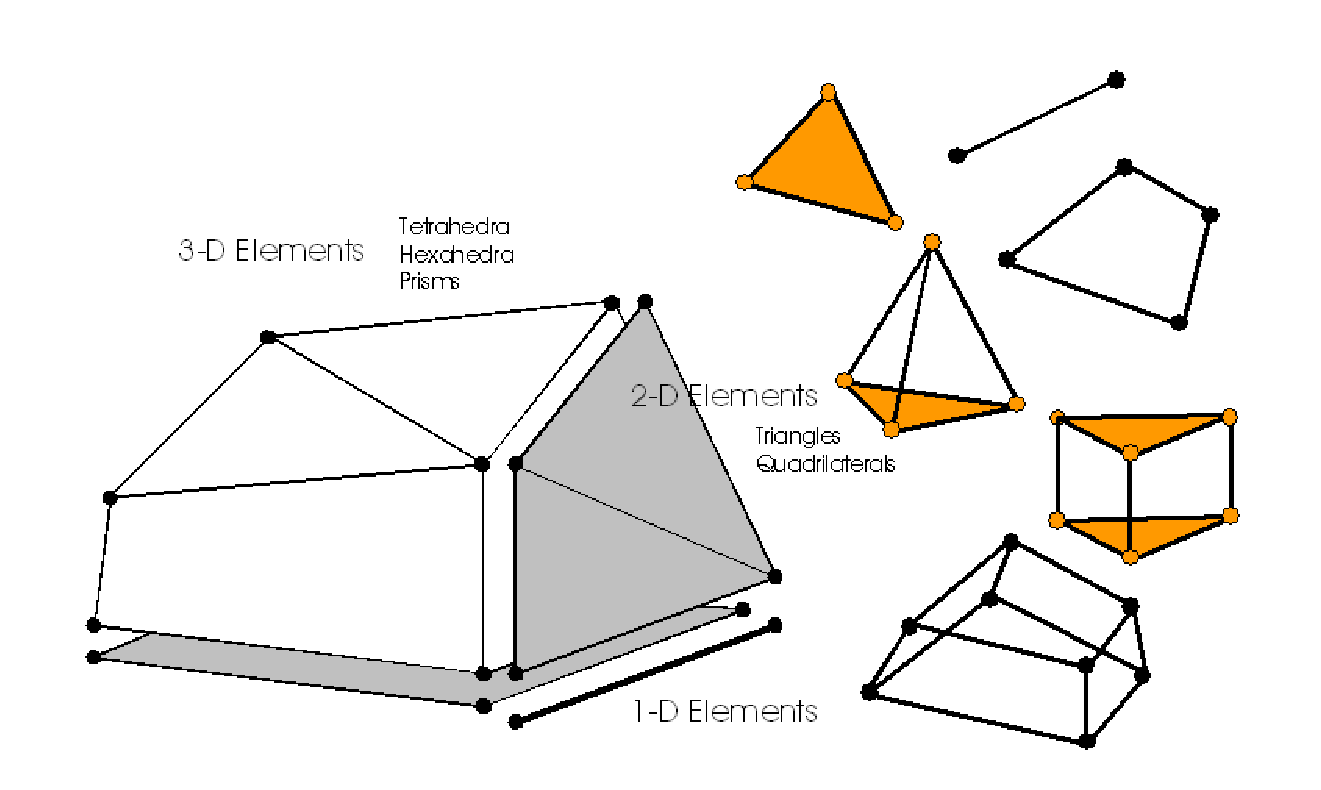
\includegraphics[scale=0.55]{figures/elements.eps}
\caption{Geometric elements types} \label{fig:ele_types}
\end{figure}

\subsection{Finite element object -- ELE-FEM}
\label{sec:ele_fem}

In this section we present the design of the finite element object, 
i.e. properties and methods, which are required to conduct the finite 
element analysis. In particular, we discuss the implementation of 
steps 2 and 3 described in  Table 
\ref{tab:alg1}, i.e., local element assembly and global assembly of system 
equation.

%In the present study, we consider the node based finite element
%and numerical integration of local finite element calculations.

%One of the advantages of object oriented programming is data
%encapsulation. In the encapsulation sense, all data, i.e.
%information, of an object are arranged to live in a scope only.
%This guarantees the safety of data within the running of
%corresponding programme as much as possible.

According to the principles of object-oriented programming, we
encapsulate common data and functionalities of finite elements into 
a base class. There are two general tasks of the finite element 
object. First, local finite element calculations and, second, 
contributions of the element to the global equation system.
%
Afterwards, we derive specific finite element objects for
different problem types (i.e. PDE types) in the framework of THM
porous media mechanics (see Fig. \ref{fig:ele_concept}).

\emph{Finite element base class:}
%
Local element calculations require the selection of specific
interpolation functions as well as their derivatives at
integration points corresponding to different element types.
Therefore, element interpolation functions are regarded as basic
items of the finite element object.
%
%We consider element interpolation functions of all kinds of
%geometric element types as global functions that are visible
%through the whole code.
%
These interpolation functions have two arguments: first, values of
shape functions or the derivative of shape functions; second,
reference points, e.g. Gauss points.
%The values of this first argument is calculated with coordinates
%of a reference point coordinates passed in through the second
%argument.
Therefore, for each kind of geometric element type, we have four
functions associated with element interpolation as

%%\small
\begin{verbatim}
  void ShapeFunctionXXXX(double*,double*);
  void ShapeFunctionHQXXXX(double*,double*);
  void GradShapeFunctionXXXX(double*,double*);
  void GradShapeFunctionHQXXXX(double*,double*);
\end{verbatim}
%%\normalsize

where \texttt{XXXX} is specifying the different geometric element
types. \texttt{ShapeFunction\-XXXX} provides linear interpolation
functions $\Sh_1$, whereas \texttt{ShapeFunctionHQXXXX} gives
quadratic interpolation functions $\Sh_2$, mentioned in section
\ref{sec:fem}. \texttt{GradShape\-FunctionXXXX} and
\texttt{GradShapeFunctionHQXXXX} offer the derivatives of the
corresponding interpolation functions $\Sh_1$ and $\Sh_2$,
respectively. Interpolation functions for all kinds of element types are declared as global functions. 
The function pointer 
\texttt{void (*VoidFuncDXCDX) (double*,double*)}
is defined to point to the addresses of the global interpolation 
functions. 
 The C++ implementation of the finite element base class \texttt{CElement} is 
given in Fig. \ref{fig:fem_root}.

\begin{figure}[htb!]
\centering
\shadowbox{
\begin{minipage}{\textwidth}
\scriptsize
\begin{verbatim}
class CFiniteElement {
  protected: // Member data
    CElem* m_ele_geo; // Instance of geometric element
    int order; //Order of shape functions
    int n_gauss_points; // Number of Gauss points
    int n_gauss; // Number of sample points for Gauss integration
    mutable double unit[4]; // Local element coordinates
    double* Jacobian; // Jacobian matrix
    double* invJacobian; // Inverse Jacobian matrix
    double* shape_fct; // Linear shape function values at Gauss points
    double* shape_fct_HQ; // Quadratic shape function values at Gauss points
    double* d_shape_fct; // Linear shape function derivative values at Gauss points
    double* d_shape_fct_HQ; // Quadratic shape function derivative values at
                            // Gauss points
  public: // Member functions
    CFiniteElement(const int order=1);
    virtual ~CFiniteElement();
    virtual void Config(CElem* m_ele_geo);
    virtual void ConfigNumerics(const int type);
    double GetGaussData(const int gp,int& gp_r,int& gp_s,int& gp_t)
    virtual void ComputeShapeFct(const int order);
    virtual void ComputeGradShapeFct(const int order);
    virtual double ComputeJacobian(const int order);
    virtual void RealCoordinates(double*xyz);
    virtual void RefCoordinates(double*xyz);
    virtual void LocalAssembly();
    virtual void FaceIntegration();
  protected: // Member functions
    VoidFuncDXCDX ShapeFunction; // Prototype for linear shape functions
    VoidFuncDXCDX ShapeFunctionHQ; // Prototype for quadratic shape functions
    VoidFuncDXCDX GradShapeFunction; // Prototype for linear shape function derivatives
    VoidFuncDXCDX GradShapeFunctionHQ; // Prototype for quadratic shape 
                                       // function derivatives
}
\end{verbatim}
\normalfont\normalsize

\end{minipage}
}
\caption{Finite element base class}
\label{fig:fem_root}
\end{figure}

Member variable, \texttt{m\_ele\_geo}, is a pointer to the
corresponding geometric element object \texttt{CElem}, which links
the finite element object to geometry. When the local assembly
takes place for an element, the instance of this element is
obtained by finite element object with its member function,
\texttt{void Config(CElem\* m\_ele\_geo)}. With this, the finite
element object has all geometrical and topological properties such as geometric type,
coordinate nodes, neighbors for local element calculation.

%Element configuration is based on the geometric element type. The
%C++ implementation of the \texttt{Config} function is presented in
%Fig. \ref{fig:fem_num}.
%
%\input{code/fem_num}

Different weak forms arise from the different governing equations
of flow problem, heat transport problem and mechanical problem
(eqn. (\ref{eq:wkmass}), (\ref{eq:wkhTmass}) and
(\ref{eq:wkstress})). This requires different element level
computations for the specific problem. Since root finite element
object provides the basic numerical functionality, we can use 
this object directly for the benefit of the polymorphism mechanism
of object oriented programming.


%=========================================================================
\subsection{Process related finite element objects -- ELE-PCS}
\label{sec:ele_pcs}

Only at this stage (last part of element object concept) we
introduce process-related data. The element object
\texttt{CFiniteElementPCS} should work for all processes: fluid
flow, heat transport, deformation and reaction processes
regardless of PDE type and type of unknown field functions (scalar
or vector quantities).

The finite element object ELE-PCS has two tasks: First, calculation 
of element matrices, which are formed by shape functions 
($\Sh_1,\nabla\Sh_1$) and process-specific material properties 
(\texttt{MAT} objects) (Step 2 in Table \ref{tab:alg1}). Second, 
provide local element contributions to the global equation system: 
$A_{ij} x_i = b_j$, where $i,j$ are global node indices (Step 3 in 
Table \ref{tab:alg1}).

The C++ implementation of the process-related finite element
object ELE-PCS is given in Fig. \ref{fig:fem_one}.

\begin{itemize}
%.........................................................................
 \item ELE-FEM relation:
Process related instances are derived from the finite element base
class \texttt{CFiniteElement}. Therefore, they inherit all
necessary geometric and topological data from ELE-GEO, ELE-FEM,
and ELE-MSH objects.
%.........................................................................
 \item PCS relation:
Process related finite element objects need a reference to the
related PCS instance, which is conducted by the ELE-PCS class
constructor.
%.........................................................................
 \item MAT relations:
References to all \texttt{MAT} objects, i.e.
\texttt{CFluidProperties* m\_mfp}, \texttt{CSolidProper\-ties*
m\_msp} and \texttt{CMediumProperties* m\_mmp}, are used to get
the required material parameters of the specified
process(\texttt{CProcess* m\_pcs}). Member function
\texttt{SetMaterial()} prepares the references to process-specific
material properties to accelerate later computations. This insures
that the ELE-FEM objects works properly for all THM processes,
i.e. fluid flow, heat transport and deformation.
%.........................................................................
 \item Local assembly - Element matrices:
Based on geometric and finite element base data (ELE-FEM relation)
and the references to material data (PCS-MAT relation) the
process-specific element matrices can be calculated now
(\texttt{CalcXXXXMatrix()}). Member functions are used to
calculate the material coefficients in the Gauss integration
points (\texttt{CalcXXXXMatrixCoefficients()}). They are defined
as \texttt{inline} types to improve the computation efficiency.
Local element matrices and vectors are stored in the corresponding
symmetric/unsymmetric matrix and vector constructs.
%.........................................................................
 \item Global assembly - Equation system:
The global assembly is conducted by the \texttt{Assemble()}
function. It updates the individual element contributions in the
equation system, i.e. global left-hand-side (LHS) matrix
($A_{ij}$) and global right-hand-side (RHS) vector ($b_j$). To
this purpose the assembly functions needs the relations between
local element node and global mesh node numbers, which is provided
by the ELE-MSH topology (section \ref{sec:ele_msh}).
\texttt{Assemble()} functions are available for different PDE
types. How the \texttt{Assemble()} is implemented for a parabolic
PDE is shown in Fig. \ref{fig:fem_asm}.
\end{itemize}

\begin{figure}[htb!]
\centering
\shadowbox{
\begin{minipage}{\textwidth}
\footnotesize
\begin{verbatim}
class CFiniteElementPCS::public CFiniteElement {
  private: // Member data
    // PCS relation
    CProcess* m_pcs;
    // MAT relations
    CFluidProperties* m_mfp;
    CSolidProperties* m_mfp;
    CMediumProperties* m_mmp;
    // Element matrices
    SymMatrix* MassMatrix;
    SymMatrix* LaplaceMatrix;
    SymMatrix* PressureCouplingMatrix;
    Matrix*    AdvectionMatrix;
    Matrix*    StrainMatrix;
    Matrix*    StrainCouplingMatrix;
    ...
    Matrix*    LHSMatrix;
    Vec*       RHSVector;
  public:  // Member functions
    // Construction
    CFiniteElementPCS(CProcess* m_pcs);
    ~CFiniteElementPCS();
    // MAT functions
    void SetMaterial();
    inline void CalcMassMatrixCoefficient();
    inline void CalcAdvectionMatrixCoefficient();
    inline void CalcLaplaceMatrixCoefficient();
    inline void CalcStrainMatrixCoefficient();
    inline void CalcStrainCouplingMatrixCoefficient();
    inline void CalcPressureCouplingMatrixCoefficient();
    // Element matrices
    inline double InterpolateGPValues(double*); // Interpolation at Gauss points
    void SetMemory();
    void CalcMassMatrix();
    void CalcLumpedMassMatrix();
    void CalcAdvectionMatrix();
    void CalcLaplaceMatrix();
    void CalcStrainMatrix();
    void CalcStrainCouplingMatrix();
    void CalcPressureCouplingMatrix();
    void CalcGravityVector();
    void LocalAssembly(); // LHS element contribution
    ...
    // Element contribution to global equation system
    void GlobalAssembly(); // LHS matrix contribution
}
\end{verbatim}
\normalfont\normalsize

\end{minipage}
}
\caption{Process related finite element class}
\label{fig:fem_one}
\end{figure}


\begin{figure}[H]
\centering
\shadowbox{
\begin{minipage}{0.7\textwidth}
\small
\begin{verbatim}
void CFiniteElementPCS::AssembleParabolicPDEType()
{
  // MAT relations
  SetMaterial();
  // Calculation and assembly of element matrices
  CalcMassMatrix();
  CalcLaplaceMatrix();
  CalcStrainCouplingMatrix();
  // Calculation and assembly of RHS vector
  CalcRHSVector();
}
\end{verbatim}
\normalfont\normalsize

\end{minipage}
}
\caption{Linear element assemble function}
\label{fig:fem_asm}
\end{figure}

%-------------------------------------------------------------------------
%\subsubsection{Finite element objects for vector field functions}

%Deformation process is governed by the Navier's equation. The
%local element matrices like tangential matrix (\ref{eq:Tang}) has
%different expression in addition to those arise from the Laplace
%type equations. Moreover, the non-linear analysis of such problems
%involving complex local calculation. To this purpose, a
%corresponding finite element object is derived from root finite
%element object.
%The C++ implementation of the quadratic FEOs for
%deformation problems is given in Fig. \ref{fig:fem_dm}.

%\input{code/fem_dm.tex}

%In addition to the standard finite element object defined in section
%\ref{sec:finone}, this class needs a reference to solid material
%properties.

%The solid phase material object (\texttt{MSP}) provides the
%constitutive stress-strain relationships for linear as well as
%nonlinear behavior. While fluid material object allows deformation
%finite element object incorporate the coupling calculation.

%Element stiffness matrix, eqn. (\ref{eq:Tang}), pressure coupling
%matrix, eqn. (\ref{eq:CMatrix}), and RHS vector are calculated by
%member function \texttt{LocalAssembly} and assembled to the global
%equation system by member function \texttt{GlobalAssembly}.
%Modified local assemble functions are required for enhanced strain
%element calculations.

\subsection{Element-Mesh relations -- ELE-MSH}
\label{sec:ele_msh}

From Fig. \ref{fig:ele_objects} it can be seen, that element-mesh
relations have multiple functions in the element concept, e.g.
\begin{itemize}
 \item ELE-GEO relation: mesh topology, neighbor relationships of
 geometric elements, element connectivity, incorporation of of boundary
 conditions,
 \item ELE-FEM relation: coordinate transformation between local
 element and global coordinates,
 \item ELE-PCS relation: local element nodes and node index in the
 global equation system, material domains.
\end{itemize}

\subsubsection{ELE-GEO relation}

Apart from the individual/intrinsic element properties, the
\texttt{ELEM} object contains information about mesh topology,
i.e. how this element is emplaced in the element mesh. For
instance, the (\texttt{sub\_domain}) index indicates the part of
the domain to which this element belongs. This number is used e.g.
to distinguish elements in different areas of the domain with
different material properties. Neighbor relationships of geometric
elements are important topological properties of an element mesh.
Neighbors of an element are all those elements adjacent to the
faces of the element. Since the definition of \texttt{ELEM} object
provides necessary functionality of different geometric element
types, we use pointers to \texttt{ELEM} object itself to recode
neighbors as

\texttt{Vector$<${}CElem$\ast>${}\ neighbors;}

\begin{figure}[H]
 \centering
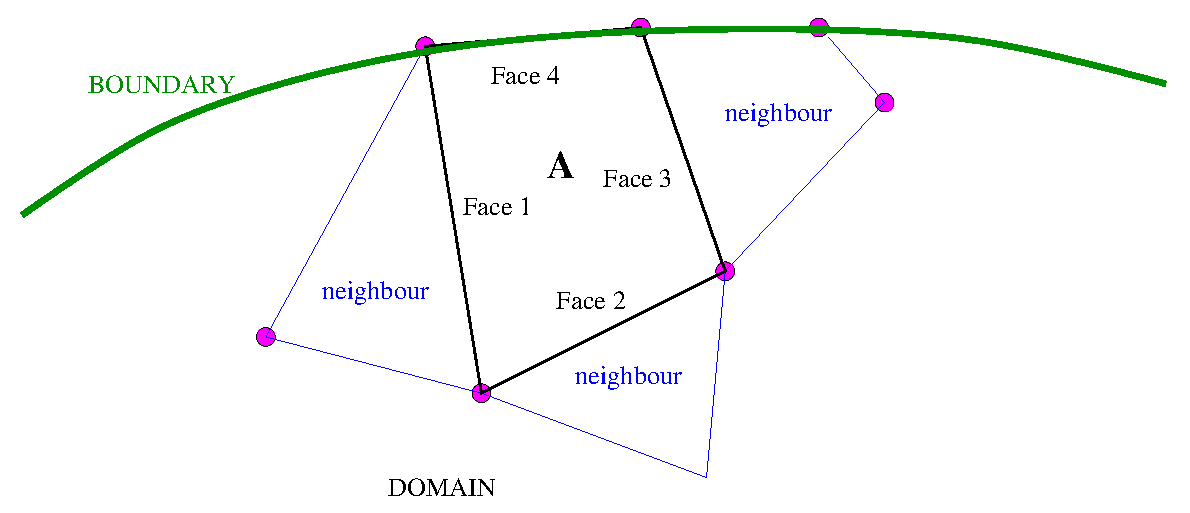
\includegraphics[scale=0.6]{figures/neighbor.eps}
\caption{Definition of element neighbors} \label{fig:gnei}
\end{figure}

As an example Fig. \ref{fig:gnei} illustrates the arrangement of
neighbor relationships in 2D space, in which quadrilateral
element A has three neighbor elements adjacent to its faces (i.e.
edges in 2D) 1, 2 and 3. Neighbors 1 and 2 are triangle elements,
while neighbor 3 is a quadrilateral element. Face 4 is on the
domain boundary, which is not shared by any other element. Vector
member, \texttt{neighbors}, is initialized with size of 4 and
assigned during mesh construction. The first three entries are
assigned with pointers to neighbors 1, 2 and 3. The last entry of
the vector is filled with a pointer to a surface (Face 4), which
is an instance of \texttt{ELEM} object configured for a line
element. The boundary type \texttt{position} of this instance is
set as 'B'. The coding of the element neighboring process is given
below:

\small
\begin{center}
\begin{verbatim}
neighbors[0] = (CElem*) Neighbour1;
neighbors[1] = (CElem*) Neighbour2;
neighbors[2] = (CElem*) Neighbour3;
neighbors[3] = (CElem*) Face4;
Face4->position = 'B'; // on domain boundary
Face4->owner = this; // this element
\end{verbatim}
\end{center}
\normalsize

The above neighbor vector is a member of element,
i.e., ELEM, object.

\subsubsection{ELE-FEM relation}

The ELE-FEM association concerns coordinate transformation between
local element and global coordinates. Depending on the geometric
and numerical type of a finite element, related shape functions
and their derivatives are available (section \ref{sec:ele_fem}).
%%This is particularly important for hybrid meshes (Fig.
%%\ref{ffig:gnei}). 
Jacobian calculations are another typical ELE-FEM methods.

\subsubsection{ELE-PCS relation}

Subdomain properties of element are used to describe heterogeneity, 
i.e. local variation of material properties for different problems. 
Element neighbor relationships are essential data for constructing 
the mesh and determine the propagation orientation of 
discontinuities in failure analysis (section \ref{sec:apl_m}). 
Moreover, the proposed element concept allows the assignment of 
different processes (PCS objects) and meshes (MSH objects). 
%%This is an important feature for upscaling procedures \cite{Kol:2005b}.


%\include{example}
%\include{cons}

\begin{itemize}
	\item sparse objects (Wang 2009)
	\item parallelization (Wang et al. 2009)
	\item XFEM (Watanabe 2010)
\end{itemize}